% Created 2018-06-01 Fri 17:41
\documentclass[a4paper,11pt]{report}
                % input
                \usepackage[utf8]{luainputenc}
                \usepackage{fontspec}
                \usepackage{unicode-math}
                \usepackage[novoc]{arabluatex}
                \newfontfamily\arabicfont[Script=Arabic]{Scheherazade}
                \newcommand{\arbt}[1]{{\Large{\arb{#1}}}} %{\arbt{...}}
                \newcommand{\arbT}[1]{{\LARGE\arb{#1}}} %\arbT{...}
                % layout
                \usepackage{layout}
                \usepackage{setspace} %package pour les interlignes
                \usepackage{multicol}
                \setlength{\columnsep}{40pt}
                \usepackage{xcolor} % package pour les couleurs
                % headers ...
                \usepackage{fancyhdr} % header etc
                \usepackage{fancybox} %package pour les encadrements supp
                \pagestyle{fancy} % Use en-tetes et des pieds de page personnaliser grâce fancyhdr
                \usepackage[Glenn]{fncychap}
                \fancyhead[L, R, C]{} % définition en-tête
                \fancyfoot[L, R]{} % définition pied de page
                \fancyfoot[C]{\thepage}
           		\renewcommand{\headrulewidth}{0pt} % ligne haut out
	        	\renewcommand{\footrulewidth}{0pt} % ligne bas out
                % others
                \usepackage{float}
                \usepackage{array, makecell} %pour les tableaux et makecell pour les cellules
                \usepackage{multirow} %pr tableau
                \newcolumntype{P}[1]{>{\centering\arraybackslash}m{#1}} %P{taille}
                % maths
                \usepackage{amsmath, amsthm} %package pour les maths
                \usepackage{lettrine}
                \usepackage{marvosym} %package de symbole
                % others
                \usepackage{wrapfig} % pour les capsules in text
                %defaut emacs packages
                \usepackage{fixltx2e}
                \usepackage{graphicx}
                \usepackage{longtable}
                \usepackage{float}
                \usepackage{wrapfig}
                \usepackage{rotating}
                \usepackage[normalem]{ulem}
                \usepackage{textcomp}
                \usepackage{wasysym}
                \usepackage{hyperref}

               

\usepackage[top=2cm, bottom=2cm, left=2cm, right=2cm]{geometry}
\author{Ousseynou Gueye}
\date{\today}
\title{\textbf{Rapport de stage L3 \\ Laboratoire ERTIM}}
\hypersetup{
  pdfkeywords={},
  pdfsubject={A description of how I currently use org-mode},
  pdfcreator={HK}}
\begin{document}

\maketitle
\setcounter{tocdepth}{3}
\tableofcontents

\chapter{Définition des objectifs et description du corpus}
\label{sec-1}

Étude de  \emph{l'évolution de certaines formes interpellatives dans un texte arabe (le Coran) selon un découpage chronologique (les deux grandes périodes de sa révélation} (mecquoise et médinoise)). \\


\section{Présentation et Constitution du corpus}
\label{sec-1-1}

Notre corpus est constitué du texte coranique. \\

\textbf{NB} : le choix du corpus, ainsi que le travail qui va suivre n'ont aucun but religieux. Notre texte nous intéresse avant tout pour sa valeur littéraire. \\

\subsection{Pourquoi ce corpus ?}
\label{sec-1-1-1}

Pour au moins deux raisons : \\
\begin{itemize}
\item c'est un corpus large mais assez restreint pour être étudiés. \\
\item c'est un corpus connu avec des études depuis des siècles. \\
\end{itemize}

\subsection{Description du corpus}
\label{sec-1-1-2}

Le corpus est composé de : \\
\begin{itemize}
\item 114 chapitres de longueur très variables (de 3 à 286 versets). \\
\item Ces chapitres sont réparties en deux parties, correspondant aux 22 ans de sa révélation : mecquoise (610-622), médinoise (622-632). \\

\item Environ 85 000 mots graphiques. \\

\item 349 formules interpellatives commençant par \textbf{\arbt{يا}} qui est l'outil du vocatif en arabe. \\
\end{itemize}


\subsection{Choix de normalisation}
\label{sec-1-1-3}

\begin{itemize}
\item Nous avons enlevé tous les signes de vocalisation. Pour une étude plus poussée, peut-être seraient-ils importants, mais dans notre cas, ils nous ajoutent des contraintes non-justifiées. \\

\item Les formules interpellatives sont toujours formées d'au moins deux mots graphiques. Or les calculs de spécificités ne se font que sur un mot graphique, donc nous avons remplacer des formules par des lettre selon le schéma suivant : \\
\end{itemize}


\begin{center}
\begin{tabular}{lllr}
Formule arabe & remplacé par : & Trad formule & Nombre\\
\hline
\arbt{يا أيّها النّاس} & A & Ô vous les hummains & 8\\
\arbt{يا أيّها الّذين آمنوا} & B & Ô vous qui croyez & 89\\
\arbt{يا أيّها النّبيّ} & C & Ô Toi le Prophète & 13\\
\arbt{يا أيّها} + x & D & Ô & 17\\
\arbt{يا أهل الكتاب} & E & Ô vous les gens du livre & 12\\
\arbt{يا} & non-remplacée & Ô & 189\\
\hline
\end{tabular}
\end{center}

\section{Hypothèse principale}
\label{sec-1-2}

Nous pensons que la formule \emph{(Ô vous les humains - \textbf{A})} devrait être caractéristique de la 1ere période, car étant au début de la révélation, il n'y pas de communauté, là où l'on devrait voir plus de \emph{(Ô vous qui croyez - \textbf{B})} à partir de la seconde période (médinoise). \\

\section{Choix des outils}
\label{sec-1-3}

Nous avons hésité et testé deux logiciels (iramuteq et TXM). \\

\subsection{Iramuteq}
\label{sec-1-3-1}

\begin{itemize}
\item Avantage : prise en charge utf8, capacité d'importer de txm. \\
\item Inconvénient : format d'entrée non pratique. Le problème peut être résolu grâce à un script, cependant il aurait fallu une longue procédure à chaque changement \\
\end{itemize}


\subsection{TXM}
\label{sec-1-3-2}

\begin{itemize}
\item Avantage : prise en charge utf8, mais surtout la capacité à utiliser un fichier csv pour les informations sur le corpus. \\
\item Inconvénient : impossibilité de changer la police, et présentation des résultats de gauche à droite, ce qui n'est pas commode pour de l'arabe. \\
\end{itemize}

\subsection{Arbitrage}
\label{sec-1-3-3}

Notre choix s'est porté sur TXM, pour l'avantage que nous avons énoncé. \\

\chapter{Résultats}
\label{sec-2}

\section{Spécificités et hypothèses de départ}
\label{sec-2-1}

Voici le premier tableau des spécificités, classées selon l'ordre alphabétique, ce qui nous permet de nous occuper de nos lettres (A - E) \\

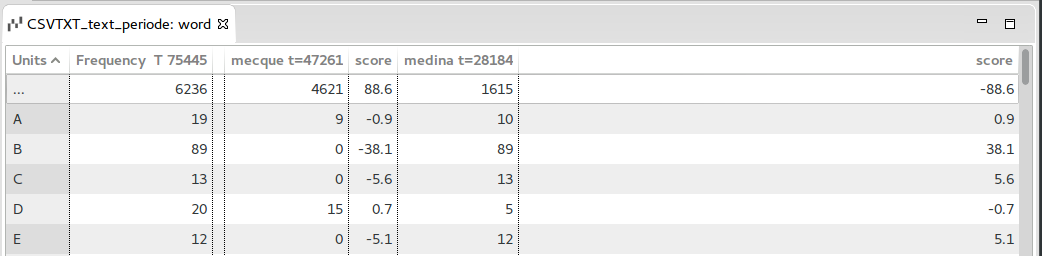
\includegraphics[width=.9\linewidth]{./img/specificites_total_1.png} \\
\begin{figure}[htb]
\centering
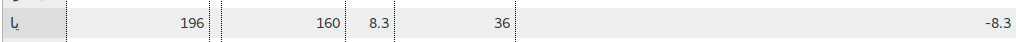
\includegraphics[width=.9\linewidth]{./img/specificites_total_2.png}
\caption{Spécifités par ordre alphabétique.}
\end{figure} \\


\subsection{Discussions et interpretation}
\label{sec-2-1-1}

\begin{enumerate}
\item Cas de A (Ô vous les humains)
\label{sec-2-1-1-1}

Notre hypothèse est invalidee, avec quasiment le même nombre d'occurence dans les deux parties (9 vs 10) \\

\uline{Lecture possible} : même ds la deuxieme partie de sa révélation, le texte coranique, qui a une vocation universelle continue de s'intéresser aux humains en général, croyants ou pas. \\

\item Cas de B (Ô vous les croyants)
\label{sec-2-1-1-2}

Notre hypothès est validée. Sur les 89 occurences dans le corpus, les 89 (100\%) se trouve dans la deuxième partie. \\

\uline{Lecture possible} : dans cette seconde partie, nous avons une communaute naissante, ce qui justifie la mention des croyants. \\
\end{enumerate}

\subsection{Ouverture}
\label{sec-2-1-2}

Après nous être penchés sur nos deux hypothèses de base, nous avons voulu aller plus loin dans l'exploration du vocabulaire de ces deux parties. \\

\section{Champ lexicaux et spécificités}
\label{sec-2-2}

Pour cela, nous allons nous intéresser à la spécifités selon son étude naturelle qui est celle du score. \\

Nous regarderons les 35 termes les spécifiques à chaque partie, tout en proposant notre explication sur les phénomènes qui nous semblent les plus intérressants. \\


\subsection{Vocabulaire mecquois}
\label{sec-2-2-1}

\begin{figure}[H]
\centering
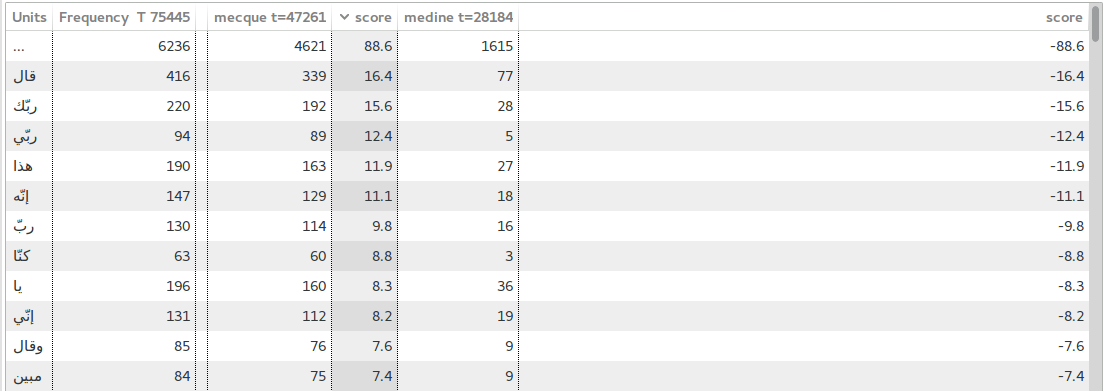
\includegraphics[width=.9\linewidth]{./img/spec_mecque_1.png}
\caption{Spécificités de la période mecquoise 1}
\end{figure} \\

\begin{figure}[H]
\centering
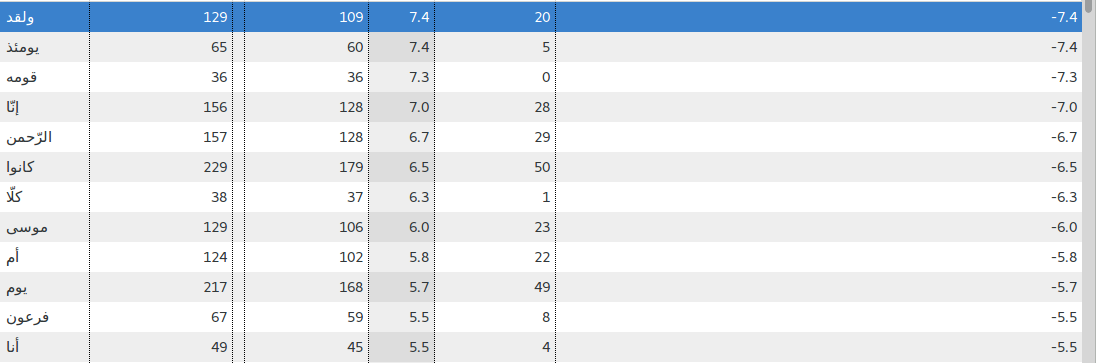
\includegraphics[width=.9\linewidth]{./img/spec_mecque_2.png}
\caption{Spécificités de la période mecquoise 2}
\end{figure} \\

\begin{figure}[H]
\centering
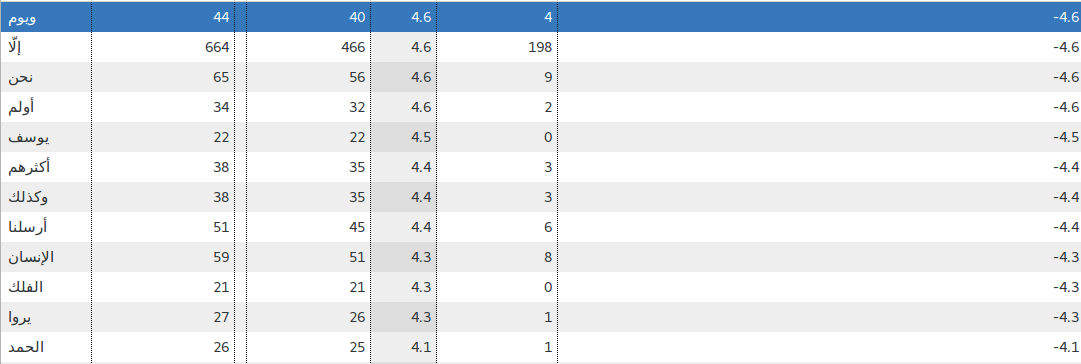
\includegraphics[width=.9\linewidth]{./img/spec_mecque_3.png}
\caption{Spécificités de la période mecquoise 3}
\end{figure} \\


\subsection{Vocabulaire médinois}
\label{sec-2-2-2}

\begin{figure}[H]
\centering
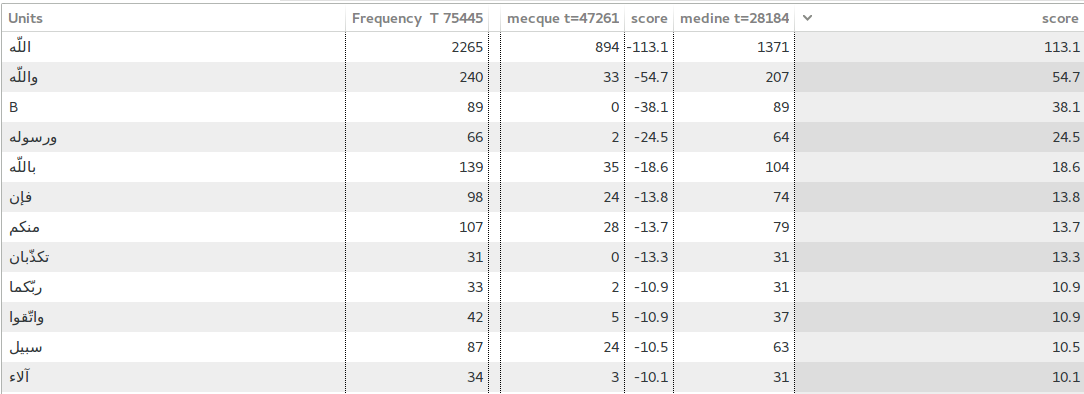
\includegraphics[width=.9\linewidth]{./img/spec_medine_1.png}
\caption{Spécificités de la période médinoise 1}
\end{figure} \\

\begin{figure}[H]
\centering
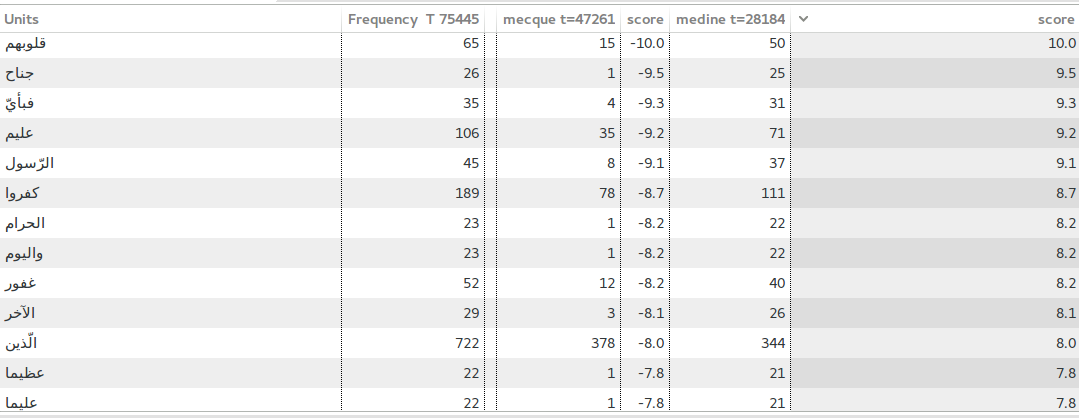
\includegraphics[width=.9\linewidth]{./img/spec_medine_2.png}
\caption{Spécificités de la période médinoise 2}
\end{figure} \\

\begin{figure}[H]
\centering
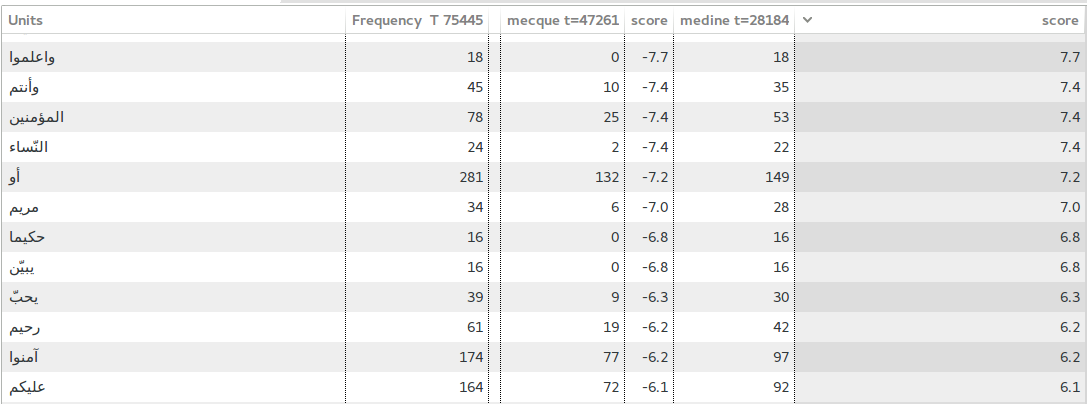
\includegraphics[width=.9\linewidth]{./img/spec_medine_3.png}
\caption{Spécificités de la période médinoise 3}
\end{figure} \\

\subsection{Analyses}
\label{sec-2-2-3}

On remarque entre autre : \\

\begin{itemize}
\item Un vocabulaire du récit privilégié dans la partie mecquoise. \\
\end{itemize}

Nous disons cela à cause de la présence de (\arbt{قال} - Il dit) présent 424 fois dans cette période soit 84.6\% des occurences totales (501). \\

\begin{itemize}
\item Un discours eschatologique accentué dans la partie mecquoise. \\
\end{itemize}

On voit que les termes (\arbt{اليوم} et \arbt{يومئذ}) faisant référence à la fin des temps et le jugement dernier apparaissent à 81\% (228/282) dans la partie mecquoise. \\

\begin{itemize}
\item Une variation de personne \\
\end{itemize}

La période mecquoise est caractérisé par plusieurs termes renvoyant à la première personne (singulier ou pluriel) comme (\arbt{كنّا} - nous sommes), (\arbt{إني}, \arbt{أنا}, \arbt{نحن} - pronoms personnels). \\

Par contre, dans la période médinoise, les termes renvoient à la deuxième ou troisième personne. Notons juste les verbes à l'impératif (\arbt{اعلموا}- sachez, \arbt{اتقوا} - ayez crainte/foi). \\

Pouvons-nous y voir un déplacement de sujet. Si la révélation commence par présenter Dieu qui parle à la première personne, l'accent est ensuite mis sur la communauté, les gens donc le non-je. \\

\begin{itemize}
\item L'évolution de l'appellation de la même entité (Dieu). \\
\end{itemize}

Dans la partie mecquoise, nous avons la présence du mot (\arbt{ربّ} - Seigneur) accompagné de pronoms personnels (Ton, mon, votre \ldots{}) 359 fois soit 83 \% des occurences (432). \\

Puis le terme semble évolué. De (Seigneur - \arbt{ربّ}) on glisse vers le mot (\arbt{الله}). On voit que 63\% (1682/2644) des occurrences ont lieu dans la partie médinoise. \\

Si le premier est plus intime, affectueux comme appelation, on passe dans le second cas a un terme neutre voire institionel. \\

\begin{itemize}
\item Un vocabulaire montrant une communauté et ses différents interlocuteurs dans la période médinoise. \\
\end{itemize}

On voit apparaitre comme spécifique à la période médinoise plusieurs termes nous indiquant la présence d'une communauté : \\

D'une part le (message - \arbt{رسول}) et les (croyants - \arbt{مؤمن(ون)}) ainsi que le verbe (croire - \arbt{آمن}). De l'autre, des verbes relatifs à la négation (\arbt{كفر} - nier) ou encore (accuser de mensonge - \arbt{كذّب}). Mais aussi des particules telles que (\arbt{منكم} - de vous), (\arbt{عليكم} - sur vous). \\

\chapter{Points positifs, limites et ouvertures}
\label{sec-3}

À l'issue de ce travail, le principal à garder est à notre avis que les outils dont nous disposons en TAL peuvent servir à traiter de l'arabe. Il est certes vrai que l'analyse n'est pas encore au même niveau que pour les corpus en caractères latins (surtout au niveau de l'étiquettage morphosyntaxique), cependant en ce qui concerne la textométrie de base, les outils font le travail. \\

Quant aux limites de notre travail : \\

\begin{itemize}
\item Nous sommes conscients qu'il puisse y avoir un biais dans la réception. Au fil des siècles, les mots changent de significations, ce qui fait que nous pouvons voir un réseau de sens qui n'était pas forcément celui du public de base. Mais cela mènerait à un débat plus philosophique que technique autour de ce que H. R. Jauss appelle l'esthétique de la réception. \\

\item Dans le même sillage, la question des limites de l'interprétation se pose. Une autre personne, devant les mêmes donnés aurait probablement eu des conclusions/observations différents. \\

\item Enfin, nous n'avons analysé qu'une infime échantillon (environ 80 mots graphiques sur 15 000 soit 0.5\%). Continuer aurait renforcé/infirmé nos observations. Mais le principal n'était pas là pour ce travail ci. \\
\end{itemize}
% HK
\end{document}